\documentclass{article}
\usepackage{tikz}
\usetikzlibrary{matrix}
\usetikzlibrary{positioning}
\usepackage{fancyvrb}
\begin{document}
\section*{Raven Stare Down}

\begin{center}
  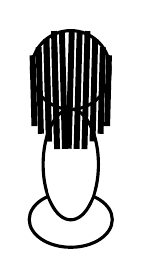
\begin{tikzpicture}
    \draw[line width=0.4mm] (0,0) circle (.5cm);
    \draw[line width=0.75mm,rotate=-1.5] (0,-1) -- (0,0.5);
    \draw[line width=0.75mm,rotate=-1.5] (0.1,-1) -- (0.1,0.5);
    \draw[line width=0.75mm,rotate=1.5] (-0.1,-1) -- (-0.1,0.5);
    \draw[line width=0.75mm,rotate=-1.5] (0.2,-1) -- (0.2,0.5);
    \draw[line width=0.75mm,rotate=1.5] (-0.2,-1) -- (-0.2,0.5);
    \draw[line width=0.75mm,rotate=1.5] (-0.3,-0.9) -- (-0.3,0.4);
    \draw[line width=0.75mm,rotate=1.5] (-0.2,-0.8) -- (-0.2,0.3);
    \draw[line width=0.75mm,rotate=1.5] (-0.4,-0.8) -- (-0.4,0.3);
    \draw[line width=0.75mm,rotate=-1.5] (0.4,-0.8) -- (0.4,0.3);
    \draw[line width=0.75mm,rotate=-1.5] (0.3,-0.9) -- (0.3,0.4);
    \draw[line width=0.75mm,rotate=1.5] (-0.3,-0.9) -- (-0.3,0.4);
    
    \draw[line width=0.75mm,rotate=1.5] (-0.48,-0.7) -- (-0.48,0.2);
    \draw[line width=0.75mm,rotate=-1.5] (0.48,-0.7) -- (0.48,0.2);
    \draw[line width=0.4mm] (0,-1.2) ellipse (10pt and 20pt);
    \draw[line width=0.4mm] (0,-1.9) ellipse (15pt and 10pt);
    %\draw[fill=white,color=white] (0,-1.9) ellipse (13pt and 8pt);
    \draw[fill=white,color=white] (0,-1.5) ellipse (8pt and 8pt);
  \end{tikzpicture}
\end{center}

\begin{center}
  \begin{tikzpicture}
    \draw[fill=white,color=white] (0,-1.5) ellipse (8pt and 8pt);
  \end{tikzpicture}
\end{center}


\begin{center}
  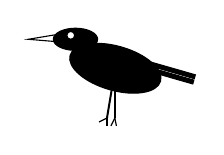
\begin{tikzpicture}
    \draw[fill=black] (0.4,-0.1) ellipse (8pt and 4pt);%(0.4,0) circle (.2cm);
    \draw (0.4,0) -- (0.4,-0.15) -- (-0.2,-0.1)-- (0.4,0);
    \draw[fill=white] (0.34,-0.05) circle(.05cm);
    \draw[rotate=-16,fill=black] (1,-0.2) ellipse (17pt and 8pt);
    \draw[rotate=-16,fill=black] (1,0) rectangle (2,-0.05);
    \draw[rotate=-16,fill=black] (1,-0.07) rectangle (2,-0.12);
    \draw[line width=0.25mm] (0.8,-1.1) -- (0.9,-0.5);
    \draw[line width=0.15mm] (0.8,-1.1) -- (0.7,-1.15);
    \draw[line width=0.15mm] (0.8,-1.1) -- (0.8,-1.2);
    
    \draw[line width=0.25mm] (0.9,-1.1) -- (0.9,-0.5);
    \draw[line width=0.15mm] (0.9,-1.1) -- (0.85,-1.2);
    \draw[line width=0.15mm] (0.9,-1.1) -- (0.92,-1.2);
    
  \end{tikzpicture}
\end{center}

Egwene faces due north
as she rests, sitting in the thick grass of Edmond's Field.
The unobstructive meadow helps her to scout out any nosy ravens
that might cast unfavorable shade on today's shearing event.

She sits unmoved
as a raven passes from behind her,
hopping westward in a straight line.

The bird is at its closest distance to Egwene at 30 WL (Westland) feet.

Unbeknownst to the raven, Egwene has a 210 degree horizontal field
of view and will see the raven as it crosses into her viewing angle.

Once the bird walks into her field of view, then the staring contest
can commence; and ultimately upon seeing Egwene's scowl
the snoopy bird will depart.

\textit{Assuming that the raven walks in a straight line
and that Egwene will only move her eyes
to reach a maximal 210 degree viewing angle},
how far in WL feet will the bird need to hop
in order for it to become visible to Egwene?


\subsection*{EOTW -1}  %\textbf{eotw -1}
\textit{ Set in The Eye of the World $>$ Earlier Ravens Prologue } \pagebreak

\section*{Heal the Corrupted Memory}

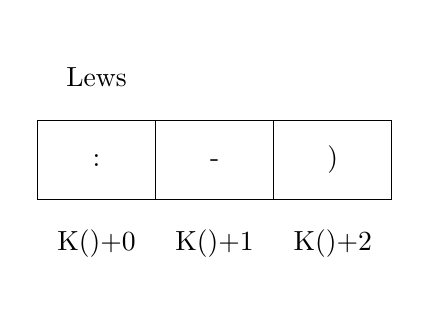
\begin{tikzpicture}
  [mat/.style={matrix of nodes,
      nodes={draw, minimum size=10mm, minimum width=15mm, anchor = north},
      column sep=-\pgflinewidth,
      row sep=0.5mm,
      nodes in empty cells,
      row 1 column 1/.style={nodes={draw=none}},
      row 1 column 2/.style={nodes={draw=none}},
      row 1 column 3/.style={nodes={draw=none}},
      row 3 column 1/.style={nodes={draw=none}},
      row 3 column 2/.style={nodes={draw=none}},
      row 3 column 3/.style={nodes={draw=none}},
  }]
  \matrix[mat] (array)
         {
           Lews  & &     \\
           :     & -     & )\\
           K()+0 & K()+1 & K()+2\\
         };
\end{tikzpicture}


\noindent 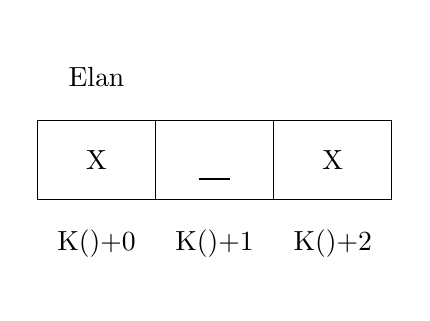
\begin{tikzpicture}
  [mat/.style={matrix of nodes,
      nodes={draw, minimum size=10mm, minimum width=15mm, anchor = north},
      column sep=-\pgflinewidth,
      row sep=0.5mm,
      nodes in empty cells,
      row 1 column 1/.style={nodes={draw=none}},
      row 1 column 2/.style={nodes={draw=none}},
      row 1 column 3/.style={nodes={draw=none}},
      row 3 column 1/.style={nodes={draw=none}},
      row 3 column 2/.style={nodes={draw=none}},
      row 3 column 3/.style={nodes={draw=none}},
  }]
  \matrix[mat] (array)
         {
           Elan  & &     \\
           X     & \raisebox{-3ex}{\underline{\hspace{0.4cm}}} & X \\
           K()+0 & K()+1                                       & K()+2\\
         };
\end{tikzpicture}


Lews Therin is joyously searching for his wife
inside his charred palace as he stands
next to the corpses of all his own kin who had met their fatal end,
and is found to be in a state of mindless bliss
as Elan Morin Tedronai appears.

As they exchange words Elan becomes aware that
Lews is ignorant to the fact that Lews had
performed this murderous act.

Lews' memory about what has happened to his kinsfolk has been corrupted.
Elan has the real memory that can be employed to heal Lews' corrupted
version of events.
Assume that the memory of the event is stored as a 3-letter happy \texttt{:-)} emoticon
in Lews' memory and can be healed by Elan's real memory,
indicated by a dead person \texttt{X\_X} emoticon.

Healing can be performed 1 letter at a time; each letter of the
emoticon components reside in their own memory unit as an adjoined sequence
in both Elan's and Lews' memory.

There are 3 magical functions that can be combined in a way
to fully heal Lews' memory.
What is the order of functions performed,
spelled out as a pronounceable spell
that will heal Lews' memory?\\
\hspace*{0.8cm}\textbf{spell: \_\ \_\ \_\ \_\ \_\ \_}

\noindent Functions:\\
\hspace*{0.2cm} - \hspace*{0.2cm}\textbf{H()} heals 1 letter memory unit at the paired position.\\
\hspace*{0.2cm} - \hspace*{0.2cm}\textbf{I()} increments the paired healing position forward 1 letter in memory.\\
\hspace*{0.2cm} - \hspace*{0.2cm}\textbf{K()} positions the paired healing position to start at the kinsfolk memory.

\subsection*{EOTW 0}
\textit{ Set in The Eye of the World $>$ Prologue Dragonmount }  \pagebreak

\section*{Solutions}

\subsection*{SLN EOTW -1}
\VerbatimInput{eotw-1.py}
\VerbatimInput{eotw-1.sln} \pagebreak

\subsection*{SLN EOTW 0}
\VerbatimInput{eotw0.py}
\VerbatimInput{eotw0.sln}


\end{document}
